% Template for PLoS
% Version 3.5 March 2018
%
% % % % % % % % % % % % % % % % % % % % % %
%
% -- IMPORTANT NOTE
%
% This template contains comments intended 
% to minimize problems and delays during our production 
% process. Please follow the template instructions
% whenever possible.
%
% % % % % % % % % % % % % % % % % % % % % % % 
%
% Once your paper is accepted for publication, 
% PLEASE REMOVE ALL TRACKED CHANGES in this file 
% and leave only the final text of your manuscript. 
% PLOS recommends the use of latexdiff to track changes during review, as this will help to maintain a clean tex file.
% Visit https://www.ctan.org/pkg/latexdiff?lang=en for info or contact us at latex@plos.org.
%
%
% There are no restrictions on package use within the LaTeX files except that 
% no packages listed in the template may be deleted.
%
% Please do not include colors or graphics in the text.
%
% The manuscript LaTeX source should be contained within a single file (do not use \input, \externaldocument, or similar commands).
%
% % % % % % % % % % % % % % % % % % % % % % %
%
% -- FIGURES AND TABLES
%
% Please include tables/figure captions directly after the paragraph where they are first cited in the text.
%
% DO NOT INCLUDE GRAPHICS IN YOUR MANUSCRIPT
% - Figures should be uploaded separately from your manuscript file. 
% - Figures generated using LaTeX should be extracted and removed from the PDF before submission. 
% - Figures containing multiple panels/subfigures must be combined into one image file before submission.
% For figure citations, please use "Fig" instead of "Figure".
% See http://journals.plos.org/plosone/s/figures for PLOS figure guidelines.
%
% Tables should be cell-based and may not contain:
% - spacing/line breaks within cells to alter layout or alignment
% - do not nest tabular environments (no tabular environments within tabular environments)
% - no graphics or colored text (cell background color/shading OK)
% See http://journals.plos.org/plosone/s/tables for table guidelines.
%
% For tables that exceed the width of the text column, use the adjustwidth environment as illustrated in the example table in text below.
%
% % % % % % % % % % % % % % % % % % % % % % % %
%
% -- EQUATIONS, MATH SYMBOLS, SUBSCRIPTS, AND SUPERSCRIPTS
%
% IMPORTANT
% Below are a few tips to help format your equations and other special characters according to our specifications. For more tips to help reduce the possibility of formatting errors during conversion, please see our LaTeX guidelines at http://journals.plos.org/plosone/s/latex

%
% For inline equations, please be sure to include all portions of an equation in the math environment.  For example, x$^2$ is incorrect; this should be formatted as $x^2$ (or $\mathrm{x}^2$ if the romanized font is desired).
%
% Do not include text that is not math in the math environment. For example, CO2 should be written as CO\textsubscript{2} instead of CO$_2$.
%
% Please add line breaks to long display equations when possible in order to fit size of the column. 
%
% For inline equations, please do not include punctuation (commas, etc) within the math environment unless this is part of the equation.
%
% When adding superscript or subscripts outside of brackets/braces, please group using {}.  For example, change "[U(D,E,\gamma)]^2" to "{[U(D,E,\gamma)]}^2". 
%
% Do not use \cal for caligraphic font.  Instead, use \mathcal{}
%
% % % % % % % % % % % % % % % % % % % % % % % % 
%
% Please contact latex@plos.org with any questions.
%
% % % % % % % % % % % % % % % % % % % % % % % %

\documentclass[10pt,letterpaper]{article}
\usepackage[top=0.85in,left=2.75in,footskip=0.75in]{geometry}

\usepackage{multirow}
\usepackage{graphicx}

% amsmath and amssymb packages, useful for mathematical formulas and symbols
\usepackage{amsmath,amssymb}

% Use adjustwidth environment to exceed column width (see example table in text)
\usepackage{changepage}

% Use Unicode characters when possible
\usepackage[utf8x]{inputenc}

% textcomp package and marvosym package for additional characters
\usepackage{textcomp,marvosym}

% cite package, to clean up citations in the main text. Do not remove.
\usepackage{cite}

% Use nameref to cite supporting information files (see Supporting Information section for more info)
\usepackage{nameref,hyperref}

% line numbers
\usepackage[right]{lineno}

% ligatures disabled
\usepackage{microtype}
\DisableLigatures[f]{encoding = *, family = * }

% color can be used to apply background shading to table cells only
\usepackage[table]{xcolor}

% array package and thick rules for tables
\usepackage{array}

% create "+" rule type for thick vertical lines
\newcolumntype{+}{!{\vrule width 2pt}}

% create \thickcline for thick horizontal lines of variable length
\newlength\savedwidth
\newcommand\thickcline[1]{%
  \noalign{\global\savedwidth\arrayrulewidth\global\arrayrulewidth 2pt}%
  \cline{#1}%
  \noalign{\vskip\arrayrulewidth}%
  \noalign{\global\arrayrulewidth\savedwidth}%
}

% \thickhline command for thick horizontal lines that span the table
\newcommand\thickhline{\noalign{\global\savedwidth\arrayrulewidth\global\arrayrulewidth 2pt}%
\hline
\noalign{\global\arrayrulewidth\savedwidth}}


% Remove comment for double spacing
%\usepackage{setspace} 
%\doublespacing

% Text layout
\raggedright
\setlength{\parindent}{0.5cm}
\textwidth 5.25in 
\textheight 8.75in

% Bold the 'Figure #' in the caption and separate it from the title/caption with a period
% Captions will be left justified
\usepackage[aboveskip=1pt,labelfont=bf,labelsep=period,justification=raggedright,singlelinecheck=off]{caption}
\renewcommand{\figurename}{Fig}

% Use the PLoS provided BiBTeX style
\bibliographystyle{plos2015}

% Remove brackets from numbering in List of References
\makeatletter
\renewcommand{\@biblabel}[1]{\quad#1.}
\makeatother



% Header and Footer with logo
\usepackage{lastpage,fancyhdr,graphicx}
\usepackage{epstopdf}
%\pagestyle{myheadings}
\pagestyle{fancy}
\fancyhf{}
%\setlength{\headheight}{27.023pt}
%\lhead{\includegraphics[width=2.0in]{PLOS-submission.eps}}
\rfoot{\thepage/\pageref{LastPage}}
\renewcommand{\headrulewidth}{0pt}
\renewcommand{\footrule}{\hrule height 2pt \vspace{2mm}}
\fancyheadoffset[L]{2.25in}
\fancyfootoffset[L]{2.25in}
\lfoot{\today}

%% Include all macros below

\newcommand{\lorem}{{\bf LOREM}}
\newcommand{\ipsum}{{\bf IPSUM}}

\newcommand{\beginsupplement}{%
        \setcounter{table}{0}
        \renewcommand{\thetable}{S\arabic{table}}%
        \setcounter{figure}{0}
        \renewcommand{\thefigure}{S\arabic{figure}}%
     }
%% END MACROS SECTION


\begin{document}
\vspace*{0.2in}

% Title must be 250 characters or less.
\begin{flushleft}
{\Large
\textbf\newline{Genetic and epigenetic study of candidate genes in mothers and embryos from pregnancy loss} % Please use "sentence case" for title and headings (capitalize only the first word in a title (or heading), the first word in a subtitle (or subheading), and any proper nouns).
}
\newline
% Insert author names, affiliations and corresponding author email (do not include titles, positions, or degrees).
\\
Valentina Aleotti\textsuperscript{1},
Amin Ravaei\textsuperscript{1},
Faisal MJ. Khan\textsuperscript{1},
Name4 Surname\textsuperscript{3},
Vincenza Colonna\textsuperscript{2},
Michele Rubini\textsuperscript{1},

%with the Lorem Ipsum Consortium\textsuperscript{\textpilcrow}
\\
\bigskip
\textbf{1} Department of Neurosciences and Rehabilitation, Section of Medical Biochemistry, Molecular Biology and Genetics, University of Ferrara, Ferrara, Italy.
\\
\textbf{2} Institute of Genetics and Biophysics, Consiglio Nazionale di Ricerche, Naples, Italy.
\\
\textbf{3} Department of Morphology, Surgery and Experimental Medicine, Section of Obstetrics and Gynecology, Ferrara, Italy.
\\
\bigskip

% Insert additional author notes using the symbols described below. Insert symbol callouts after author names as necessary.
% 
% Remove or comment out the author notes below if they aren't used.
%
% Primary Equal Contribution Note
%\Yinyang These authors contributed equally to this work.

% Additional Equal Contribution Note
% Also use this double-dagger symbol for special authorship notes, such as senior authorship.
%\ddag These authors also contributed equally to this work.

% Current address notes
%\textcurrency Current Address: Dept/Program/Center, Institution Name, City, State, Country % change symbol to "\textcurrency a" if more than one current address note
% \textcurrency b Insert second current address 
% \textcurrency c Insert third current address

% Deceased author note
%\dag Deceased

% Group/Consortium Author Note
%\textpilcrow Membership list can be found in the Acknowledgments section.

% Use the asterisk to denote corresponding authorship and provide email address in note below.
%*lttvnt@unife.it
*corresponding 


\end{flushleft}
% Please keep the abstract below 300 words
\section*{Abstract}
Pregnancy loss (PL) is defined as the fetal death within 20-28 weeks and for approximately half of the cases the cause is unknown. A number of genetic association with increased risk of PL have been described in literature, in genes related to immunity an DNA replication. In this study we investigate genetic and epigenetic associations in a cohort of mothers and embryos from 126 cases and 153 controls. We find a significant associations between increased risk of PL and the variant rs1801133 in the \textit{MTHFR} gene in the mothers and reduced risk of PL and the variant  rs2617170 in the \textit{NKG2D} in the embryos. We also found overall higher level of methylation in embryos form PL compared to control embryos from mother that did not take folic acid during pregnancy. While limited to few markers this study provide significant evidences of association of genetic markers with PL.


% Please keep the Author Summary between 150 and 200 words
% Use first person. PLOS ONE authors please skip this step. 
% Author Summary not valid for PLOS ONE submissions.   
%\section*{Author summary}


\linenumbers

\section*{Introduction}

Pregnancy loss (PL) is defined by World Health Organization as the loss of pregnancy resulting in fetal death before 20-28 weeks. Roughly 10-15 \% of all clinically recognized pregnancies result in miscarriage within the first trimester of gestation. The main known causes of PL are chromosomal anomalies, maternal factors as anatomical abnormalities, autoimmune diseases, infection diseases or advanced maternal and paternal age and environmental agents. In 50\% of cases, the causes are still unknown \cite{campana2017association, du2019polymorphisms, sudhir2016cytogenetic, oliver2014diagnosis, yakut2015chromosome}. 
\noindent Genetic association with increased risk of miscarriage have been described for several genes and in Table \ref{tab:panelofgenes} we report a synthetic description of the genes and relevant variants therein. A number of studies investigated the association between the rs1801133 (c.677C \textgreater T) and rs1801131 (c.1298A \textgreater C) polymorphisms in the gene \textit{MTHFR} and risk of PL, but the conclusions are controversial \cite{kim2006influence, biswas2008recurrent, foka2000factor}. A 14 base pair insertion/deletion in the \textit{HLA-G} gene is also considered important for fetal-maternal immune tolerance and successful pregnancy \cite{nowak2016possible, arjmand2016balance}. The \textit{ANXA5} gene codes a protein, the Annexin A5, that has a role as placental anticoagulant and it is abundantly expressed in placenta \cite{hayashi2013genotyping, zhang2017association}. The rs1800871 (c. 819C \textgreater T)  variants was studied in the \textit{IL-10} gene, that produces a key cytokine,crucial for the maintenance of maternal–fetal tolerance of its pleiotropic activities. A lower level of IL-10 can cause preterm birth, and preeclampsia \cite{su2016association,cochery2009interleukin,qaddourah201410, gu2016association}. The gene \textit{CTLA-4} is constitutively expressed on regulatory T cells and promotes maternal fetal tolerance \cite{zhang2018synergic, misra2016association}. The gene \textit{SMTH1} produces a serine hydroxyl-methyltran-ferase 1 involved in the cycle of folic acid \cite{coppede2015genetics, boyles2006neural,mckay2012genetic}. The gene \textit{PLK4} seems to play a role in the centriole duplication that can alter the result of mitosis contribuiting to mitotic-origin aneuploidy risk during human early embryo development \cite{mccoy2015common, zhang2017association}.
\noindent Finally, methylation has also a key role in pregnancy loss. The class I transposable element LINE-1 comprise approximately 17\% of the human genome \cite{lander2001initial} and therefore its methylation pattern is a surrogate marker of global DNA methylation level \cite{perrin2007specific}.
\noindent In this study we want to understand if the genetic and epigenetic profile plays a role in determining the risk of PL through the study of known genetic associations in a cohort of women and miscarried embryos. By studying allele frequencies at variable sites in candidate genes we find and increased risk of PL for carriers of the minor allele T at rs1801133 in the \textit{MTHFR} gene and a reduced risk in carriers of the minor allele G at rs2617170 in the \textit{NKG2D} gene. We also analyze methylation patterns of the LINE-1 sequence and found a significant increased methylation in embryos from PL compared to controls. This study confirms previous findings and provide a reference for further comparative studies. 




\section*{Materials and methods}
\subsection*{Data and samples collection}

In this study were analyzed data from 156 women that underwent Voluntary Termination of Pregnancy (VTP) and 91 recurrent pregnancy loss \textbf{(RPL)}, 40 first pregnancy loss \textbf{(FPL)} in a total of 131 women experiencing Pregnancy Loss (PL). The samples were provided by the Unit of Obstetrics and Gynecology at The Sant’Anna University Hospital of Ferrara, Italy, from 2016 to 2020. The inclusion criteria were: patient’s age in the range 18–42 years, gestational age within the first 12 weeks and the cohort of VTP pregnancy was composed of females that have a voluntary miscarriage until 90 days according to the Italian law. The exclusion criteria were: the presence of congenital or acquired immune deficiency syndrome/diseases, severe uterine or hormonal dysregulation, use of teratogenic drugs or immunosuppressive therapies, patients positive for infectious agents/diseases, such as HIV, hepatitis B virus, hepatitis C virus, syphilis, genetci anomalies (da mettere anche se non analizzate in tutti??) all before the sample collection. The samples were composed by the products of the conception and the relative peripheral blood of mothers. The project \textbf{G.R Reg. E/R (PRUA1GR-2013 00000220)} \textit{“Silent Intrauterine infections and early pregnancy loss”} was approved by Ethical Committee AVEC of Emilia Romagna, Italy, \textbf{(CE/FE 170475)} and was carried out in compliance with the Helsinki Declaration. All participants provided written informed consents before recruitment. Data set consists of medical data from interviews on 283 cases. In the questionnaire, there is information about mother’s age, Body Mass Index (BMI), gestational age, menarche, geographical origin, educational level, lifestyle factors (smoking, alcohol consumption, drug consumption), chronic disease, folic acid intake, obstetric and gynecologic history of mother and sister of the patient. All the data were anonymized right after data and sample collection. 

\subsection*{Genomic DNA extraction, quantification and storage}
\noindent The material of conception with relative media arrives in the laboratory in sterilized Falcon tubes of 15 ml. The selection of chorionic villi from the maternal material must be done under a laminar flow hood to preserve the sterility of the sample. The most challenging step of the protocol consists of distinguishing and separating exclusively the villi from the rest of the maternal material like placenta, and decidua. The dissection takes place under the hood using a stereomicroscope (e.g. Leica Microsystems Srl, All Microscopy and Histology, Milan, I-20142 Italy). The operator should recognize chorionic villi at the stereomicroscope and separate them from the decidua using scalpels. Then proceed to DNA extraction from chorionic villi. The peripheral blood from mothers was collected in tubes with EDTA at the same time of collection of the miscarriage material. Genomic DNA (gDNA) was extracted from chorionic villi dissected from abortion tissue specimens using QIAamp DNA Blood Mini Kit (Qiagen) in according to manufacturer protocols \textit{(QIAamp DNA Mini and Blood Mini Handbook 05/2016. Instruction Manual)}. The gDNA obtained from white blood cell (WBC) of peripheral blood samples from mothers was instead extracted using the Nucleon BACC1 (GE Healthcare UK), according to manufacturer protocols (\textit{RPN8501-PL Rev C 04/2008}). All genomic DNA was quantified using Qubit® dsDNA BR Assay Kit (Life technologies Oregon, USA). 

\subsection*{Genotyping}

\noindent The genomic DNA obtained from WBC and abortion tissue specimens were used for the genotyping of a panel of candidate gene variants with 5’- nucleus Real-Time PCR assay using allele-specific TaqMan probes. PCR conditions for all reaction were as follows: 50\si{\degree}C for 2 min, 95\si{\degree}C for 10 min and (95\si{\degree}C for 15 s, 60\si{\degree}C for 1 min) x 50 cycles. The instrument used for reading plate was Applied BioSystems ABI PRISM 7300 (Applied BioSystems, Foster City, CA). The gene HLA-G 14 bp was analyzed by a polymerase chain reaction (PCR) sequence-specific primer method (PCR-PAGE) \cite{castelli2014insights}. The amplification was performed by PCR with a GeneAmp PCR System 2700 thermal cycler (Applied Biosystems, Foster City, CA) in a 25 $\mu$L reaction mixture containing 100ng of genomic DNA, 10XPCR buffer, 50mM MgCl2, 10mM dNTPs, 20pmol of each primer and 1U of Taq polymerase (Invitrogen Co., Carlsbad, Ca). The PCR conditions comprised initial denaturation at 94\si{\degree}C for 2 min, followed by 10 cycles of denaturation at 94\si{\degree}C for 15 s, annealing at 64\si{\degree}C for 30 s and extension at 72\si{\degree}C for 30 s, then 25 cycles of denaturation at 94\si{\degree}C for 15 s, annealing at 63\si{\degree}C for 30 s and extension at 72\si{\degree}C for 30 s, and final extension at 72\si{\degree}C for 5 min. The purified PCR products size were analyzed using an 8\% polyacrylamide gel. The PCR products were visualized using silver staining.  %The product size was 224 bp for Ins/Ins (I/I) and 210 bp for Del/Del (D/D) and both 224 bp and 210 bp for Del/Ins (D/I) genotypes. 

\subsection*{Pyrosequencing}

\noindent This protocol is in accord to study of Khan MFJ. et al., 2017 \cite{khan2018evaluating}. The genomic DNA samples were next bisulfite-converted using EZ DNA Methylation-Lightning Kit (Zymo Research, Irvine, CA, USA), according to manufacturer's instructions (Instruction manual CAT. No. D5030T, ver 1.0.4). After that, the CpG islands of LINE-1 sequences were amplified by PCR. The PCR reactions were performed with a total volume of 25 $\mu$L containing: 10X PCR Buffer, 50mM MgCl2, 2.5 mM dNTPs, 10 pM Reverse Primer LINE-1, 10 pM Forward Primer LINE-1, 5U Taq-Polymerase and 2.5 $\mu$L of Bisulfite DNA. The cycling profile was composed of 27 cycles of 94 \si{\celsius} for 15 sec, 60\si{\celsius} for 30 sec and 72\si{\celsius} for 30 sec, followed by 72\si{\celsius} for 2 min. The amplicon of 147 bp was analyzed on 8\% polyacrylamide gel using silver staining. The products of PCR were sequenced by pyrosequencing using the PyroMark Q96 system (Qiagen), according to manufacturer’s instructions (PyroMark Q96 ID User Manual 01/2016). The average of LINE-1 methylation level was calculated as of the mean of the proportions of C (\%) at the 4 CpG sites analyzed, which were located at positions +306, +318, +321 and +328 (positions of the corresponding Guanine in the forward DNA strand, in relation to the first nucleotide base of the consensus promoter sequence in Genebank sequence no. X58075, position 305-331).

\subsection*{Statistical analysis}

\noindent The analyses done follows the guidelines for statistical analysis for case-control study of \textit{Clarke GM. et al.,2011} \cite{clarke2011basic}. All the statistical analyses were performed using the R studio software (R studio version 3.6.2). The Hardy-Weindberg equilbrium (HWE) was tested with "Hardy- Weinberg" package in R studio \cite{graffelman2015exploring}. Odds ratios (ORs) and 95\% confidence intervals (95\% CIs) were estimated on nine SNPs with MAF > 5-10\%.A z-test was applied, and a two-tailed p-value less than 0.05 was considered statistically significant. ORs were calculated for genotypes and alleles, assuming dominant, co-dominant and recessive genetic model. Methylation scores of the LINE-1 sequence was calculated as the average over all 4 CpG islands in a sample. The distribution of LINE-1 methylation levels were checked for normality using the Shapiro-Wilk test. For WBC samples that not departed from normality, as parametric test, an unpaired t-student test was used to test the significativity. For CV samples, we used a non parametric test called "\textit{Mann-Whitney}". A t-student test was used for WBC and Mann-Whitney for CV, to evaluate the difference of average of methylation with a stratification on several parameters included in the clinical database, the same for OR. All p-values were two sided, with a threshold for declaring statistical significance of p < 0.05. \\

% For figure citations, please use "Fig" instead of "Figure".

% Place figure captions after the first paragraph in which they are cited.
%\begin{figure}[!h]
%\caption{{\bf Bold the figure title.}
%Figure caption text here, please use this space for the figure panel descriptions instead of using subfigure commands. A: Lorem ipsum dolor sit amet. B: Consectetur adipiscing elit.}
%%\label{fig1}
%\end{figure}

% Results and Discussion can be combined.
\section*{Results}
\subsection*{Genetic association between PL and variants in candidate genes}
To determine if there is association between PL and alleles at nine single nucleotide polymorphic sites (SNPs) in eight genes previously associated with the risk of miscarriage (Table\ref{tab:panelofgenes}), we performed a case-control study \cite{clarke2011basic}. We used as cases 126 unrelated mothers experiencing PL for which genomic DNA (gDNA) was extracted from white blood cells (WBC) or embryos for which gDNA was extracted from chorionic villi (CV). As control we used 153 unrelated mothers undergoing voluntary termination of pregnancy (VTP) and their aborted embryos. Prior to association analysis we conducted quality check controls. First, genotype concordance rate of 98.42\% was estimated by genotyping twice 15\% of all samples and discordant samples were excluded form the analysis. Second we confirmed that all loci where in Hardy Weinberg equilibrium METTERE REF TABELLA. Finally SNPs with minor allele frequency (MAF) $<$5\% in the global sample were excluded. 
\noindent All the SNPs considered have two alleles, of which we refer as minor to the the least frequent in the general population according to Ensembl (Release 99, January 2020, www.ensembl.org).
\noindent For both WBC and CV, we evaluated allelic association (Table \ref{tab:Allele analysis in WBC and CV}) with reference to the minor allele. In WBC we found that the minor allele T of the rs1801133 variant in the gene \textit{MTHFR} confers 1.72 increased risk of PL (95\% CI: 1.22-2.43, p-value=0.0018). No other significant association was found in WBC. In CV we found that the minor allele G of the rs2617170 variant in the \textit{NKG2D} gene protects the embryo form PL (OR=0.64, 95\% CI: 0.44-0.95, p-value=0.025). No other association was significant.
\noindent The results of the allelic association were confirmed by genotypic association. We explored three models of disease penetrance: co-dominant, dominant, and recessive (Fig \ref{fig:orgeno}). Considering m and M the minor and major alleles, respectively, under the co-dominance model we estimated the odds ratio (OR) for the genotype mm relative to genotype MM (Table \ref{tab:Model genetic analysis in WBC and CV}). We confirmed both the association and the direction of the effects seen in the allelic association, i.e. risk for rs1801133 in WBC and protection for rs2617170 in CV. In particular for rs1801133 in \textit{MTHFR} the heterozygous genotype confers 1.6 increased odd of PL but this value is not significant, while the minor-allele-homozygous genotype significantly increase the risk of PL in WBC of 2.64 times (95\%CI: 1.33-5.22, p-value=0.004). For rs2617170 in \textit{NKG2D} the protective effect of the mm genotype is estimated to be 0.27 (95\%CI: 0.10-0.72, p-value = 0.0067). 
Under the dominance model we estimated the OR of the combined genotypes Mm and mm relative to genotype MM, while under the recessive model we estimated the OR of the genotype mm against the combined Mm and MM genotypes. For rs1801133 we confirm a significant 1.8 risk increase (95\%CI p-value ) in PL for WBC under a dominant model, whereas for rs2617170 we confirm a 0.29 decrease in risk in CV (95\%CI p-value) under a recessive model of disease penetrance.

\subsection*{Methylation pattern of the LINE-1 sequence}
We compared methylation patterns at the LINE-1 sequence between PL and VTP to determine if there are significant differences. In order to choose the appropriate test for comparison, we first determined that in the CV for both PL and VTP the fraction of methylation of LINE-1 follows a normal distribution  (Shapiro-Wilk test p-value=3.96x10\textsuperscript{-5} and p-value=0.0006, respectively), whereas in WBC it does not (Shapiro-Wilk test p-value= 0.64 for PL and  p-value= 0.080 for VTP). We observe a trend of higher methylation levels in WBC compared to CV (Fig \ref{fig:Global methylation}). Within WBC mean methylation levels are comparable between PL and VTP (Table \ref{tab:methylation level}, t-test p-value=0.7) whereas in CV LINE-1 methylation levels are significantly higher in PL compared to VTP (Table \ref{tab:methylation level}, MW test p-value=0.001).  
\noindent To further investigate the significant increase in the methylation of the LINE-1 in CV from PL compared to CV from VTP, we stratified over several parameter present in the clinical database, i.e. the  age, BMI, smoking exposure, and folic acid intake in WBC and age and sex in the CV (Table \ref{tab:LINE-1 methylation on clinical data}). We found a significant increase in methylation of LINE-1 in CV form PL deriving from WBC that did not take folic acid, compared to PL from WBC that did take folic acid during pregnancy (62\%$\pm$1\% and 57\%$\pm$0.81\%, respectively; MW-test p-value= 0.03). The same analysis in VTP was not possible as no WBC of VTP was taking folic acid.



% Place tables after the first paragraph in which they are cited.
%\begin{table}[!ht]
%\begin{adjustwidth}{-2.25in}{0in} % Comment out/remove adjustwidth environment if table fits in text column.
%%%%%%%%%%%%%%%\centering
%%%%%%%%%%%%%%\caption{
%%%%%%%%%%%%%{\bf Table caption Nulla mi mi, venenatis sed ipsum varius, volutpat euismod diam.}}
%%%%%%%%%%%%\begin{tabular}{|l+l|l|l|l|l|l|l|}
%%%%%%%%%%%\hline
%%%%%%%%%%\multicolumn{4}{|l|}{\bf Heading1} & \multicolumn{4}{|l|}{\bf Heading2}\\ \thickhline
%%%%%%%%%$cell1 row1$ & cell2 row 1 & cell3 row 1 & cell4 row 1 & cell5 row 1 & cell6 row 1 & cell7 row 1 & cell8 row 1\\ \hline
%%%%%%%%$cell1 row2$ & cell2 row 2 & cell3 row 2 & cell4 row 2 & cell5 row 2 & cell6 row 2 & cell7 row 2 & cell8 row 2\\ \hline
%%%%%%%$cell1 row3$ & cell2 row 3 & cell3 row 3 & cell4 row 3 & cell5 row 3 & cell6 row 3 & cell7 row 3 & cell8 row 3\\ \hline
%%%%%%\end{tabular}
%%%%%\begin{flushleft} Table notes Phasellus venenatis, tortor nec vestibulum mattis, massa tortor interdum felis, nec pellentesque metus tortor nec nisl. Ut ornare mauris tellus, vel dapibus arcu suscipit sed.
%%%\end{flushleft}
%%\label{table1}
%\end{adjustwidth}
%\end{table}


%PLOS does not support heading levels beyond the 3rd (no 4th level headings).
%%%\subsection*{\lorem\ and \ipsum\ nunc blandit a tortor}
%%\subsubsection*{3rd level heading} 
%Maecenas convallis mauris sit amet sem ultrices gravida. Etiam eget sapien nibh. Sed ac ipsum eget enim egestas ullamcorper nec euismod ligula. Curabitur fringilla pulvinar lectus consectetur pellentesque. Quisque augue sem, tincidunt sit amet feugiat eget, ullamcorper sed velit. Sed non aliquet felis. Lorem ipsum dolor sit amet, consectetur adipiscing elit. Mauris commodo justo ac dui pretium imperdiet. Sed suscipit iaculis mi at feugiat. 

%%%%%\begin{enumerate}
	%%%\item{react}
%%	\item{diffuse free particles}
%	\item{increment time by dt and go to 1}
%%%%\end{enumerate}


%%%\subsection*{Sed ac quam id nisi malesuada congue}

%%Nulla mi mi, venenatis sed ipsum varius, volutpat euismod diam. Proin rutrum vel massa non gravida. %Quisque tempor sem et dignissim rutrum. Lorem ipsum dolor sit amet, consectetur adipiscing elit. Morbi at justo vitae nulla elementum commodo eu id massa. In vitae diam ac augue semper tincidunt eu ut eros. Fusce fringilla erat porttitor lectus cursus, vel sagittis arcu lobortis. Aliquam in enim semper, aliquam massa id, cursus neque. Praesent faucibus semper libero.

%\begin{itemize}
%%%%	\item First bulleted item.
%%%	\item Second bulleted item.
%%	\item Third bulleted item.
%\end{itemize}

\section*{Discussion}

Genetic and epigenetic markers have been demonstrated to play an important role in miscarriage. This exploratory study suggests that the risk of PL is influenced by maternal and fetal genotype. In particular, the minor allele of \textit{MTHFR} c.677C>T seems to have an effect on the risk of PL, with triplicate risk in carriers of the minor allele homozygous genotype T/T and half risk in the heterozygous carriers. We speculate that the increased risk of PL could be related to reduced synthesis of 5- methyl-Tetrahydrofolate \cite{jacques1996relation}, which could dysregulate the methylation of gDNA, causing epigenetic modifications affecting the survival of the embryos. A study of Wilcken et al., 2003 \cite{wilcken2003geographical} on newborns around the world, shows that on southern Europeans (Spain and northern Italy) about 12-15\% of newborn had T/T genotype, with a peak in southern Italy (20-26\% in Campania and Sicily). 
\noindent Therefore, while these findings needs further investigation in a larger cohort, they already provide initial indications particulary relevant for the population of origin of the mothers enrolled in this study. 
\noindent We also found reduce the risk of PL in the embryo associated to the minor allele of rs2617170 in the gene \textit{NKG2D}. In a study from \textit{Hizem et al.,2014} \cite{hizem2014polymorphisms}, the major allele homozygous genotype AA in mothers is correlated with higher cytotoxic activity. Here for the first time we observe the effects on embryos is opposite, i.e. protection from PL. In a normal pregnancy, the role of \textit{NKG2D} is to stimulate decidual NK cells to produce a type of cytokines that induce angiogenesis and contribute to the vascular remodeling of the uterus. The maternally produced cytokines ensure the communication between the fetal trophoblast and the maternal decidual cells when the trophoblast invades the decidua. Syncytiotrophoblast cells produce and secrete NKG2D ligands via exosomes. In a normal pregnancy the exosomes interact with NKG2D and downregulate the receptor expression on PBMC causing the inhibition of the NKG2D-dependent cytotoxic response. We speculate that the minor allele in embryos contribute to maintain this secretion by the cells of the syncytiotrophoblast \cite{mei2012defects}. 
\noindent Epigenetic mechanisms are important for the development and differentiation of the embryo. They can be influenced by exogenous risk factors \cite{godderis2015global} and if disregulated during the intrauterine period can cause disease in later life \cite{breton2009prenatal}. Here we compared the DNA methylation patterns of cases and control to understand if the life style of the mothers (e.g. smoke, alcool, folic acid intake) can influence the outcome of the pregnancy. Referring to the LINE-1 methylation as a proxy for genome-wide methylation, we found significant higher methylation levels in PL compared VTP in the embryos (CV) and when stratifying by risk factor we observe a correlation with lack of periconceptional supplementation with folic acid in the mothers. This results, although preliminary, suggest that modification of the epigenetic profiles of the embryo could play a role in determining the pregnancy loss. Folate is an important precursor of one-carbon units required for DNA methylation and folate metabolism alteration are associated to epigenetic alterations in cancer \cite{jin2009different}. 

\section*{Conclusion}

In conclusion we investigated genetic and epigenetic association with pregnancy loss confirming known risk and protective factors. These indication can be relevant to develop better diagnostic tools. In the future we would like to extend the analysis to a larger number of markers and to complete trios. 

%\section*{Supporting information}
% Include only the SI item label in the paragraph heading. Use the \nameref{label} command to cite SI items in the text.
%\paragraph*{S1 Fig.}
%\label{S1_Fig}
%{\bf Bold the title sentence.} Add descriptive text after the title of the item (optional).

%\paragraph*{S2 Fig.}
%\label{S2_Fig}
%{\bf Lorem ipsum.} Maecenas convallis mauris sit amet sem ultrices gravida. Etiam eget sapien nibh. Sed ac ipsum eget enim egestas ullamcorper nec euismod ligula. Curabitur fringilla pulvinar lectus consectetur pellentesque.

%\paragraph*{S1 File.}
%\label{S1_File}
%{\bf Lorem ipsum.}  Maecenas convallis mauris sit amet sem ultrices gravida. Etiam eget sapien nibh. Sed ac ipsum eget enim egestas ullamcorper nec euismod ligula. Curabitur fringilla pulvinar lectus consectetur pellentesque.

%\paragraph*{S1 Video.}
%\label{S1_Video}
%{\bf Lorem ipsum.}  Maecenas convallis mauris sit amet sem ultrices gravida. Etiam eget sapien nibh. Sed ac ipsum eget enim egestas ullamcorper nec euismod ligula. Curabitur fringilla pulvinar lectus consectetur pellentesque.

%\paragraph*{S1 Appendix.}
%\label{S1_Appendix}

%\paragraph*{S1 Table.}
%\label{S1_Table}

\section*{Acknowledgments}


\begin{figure}[!ht]
    \centering
    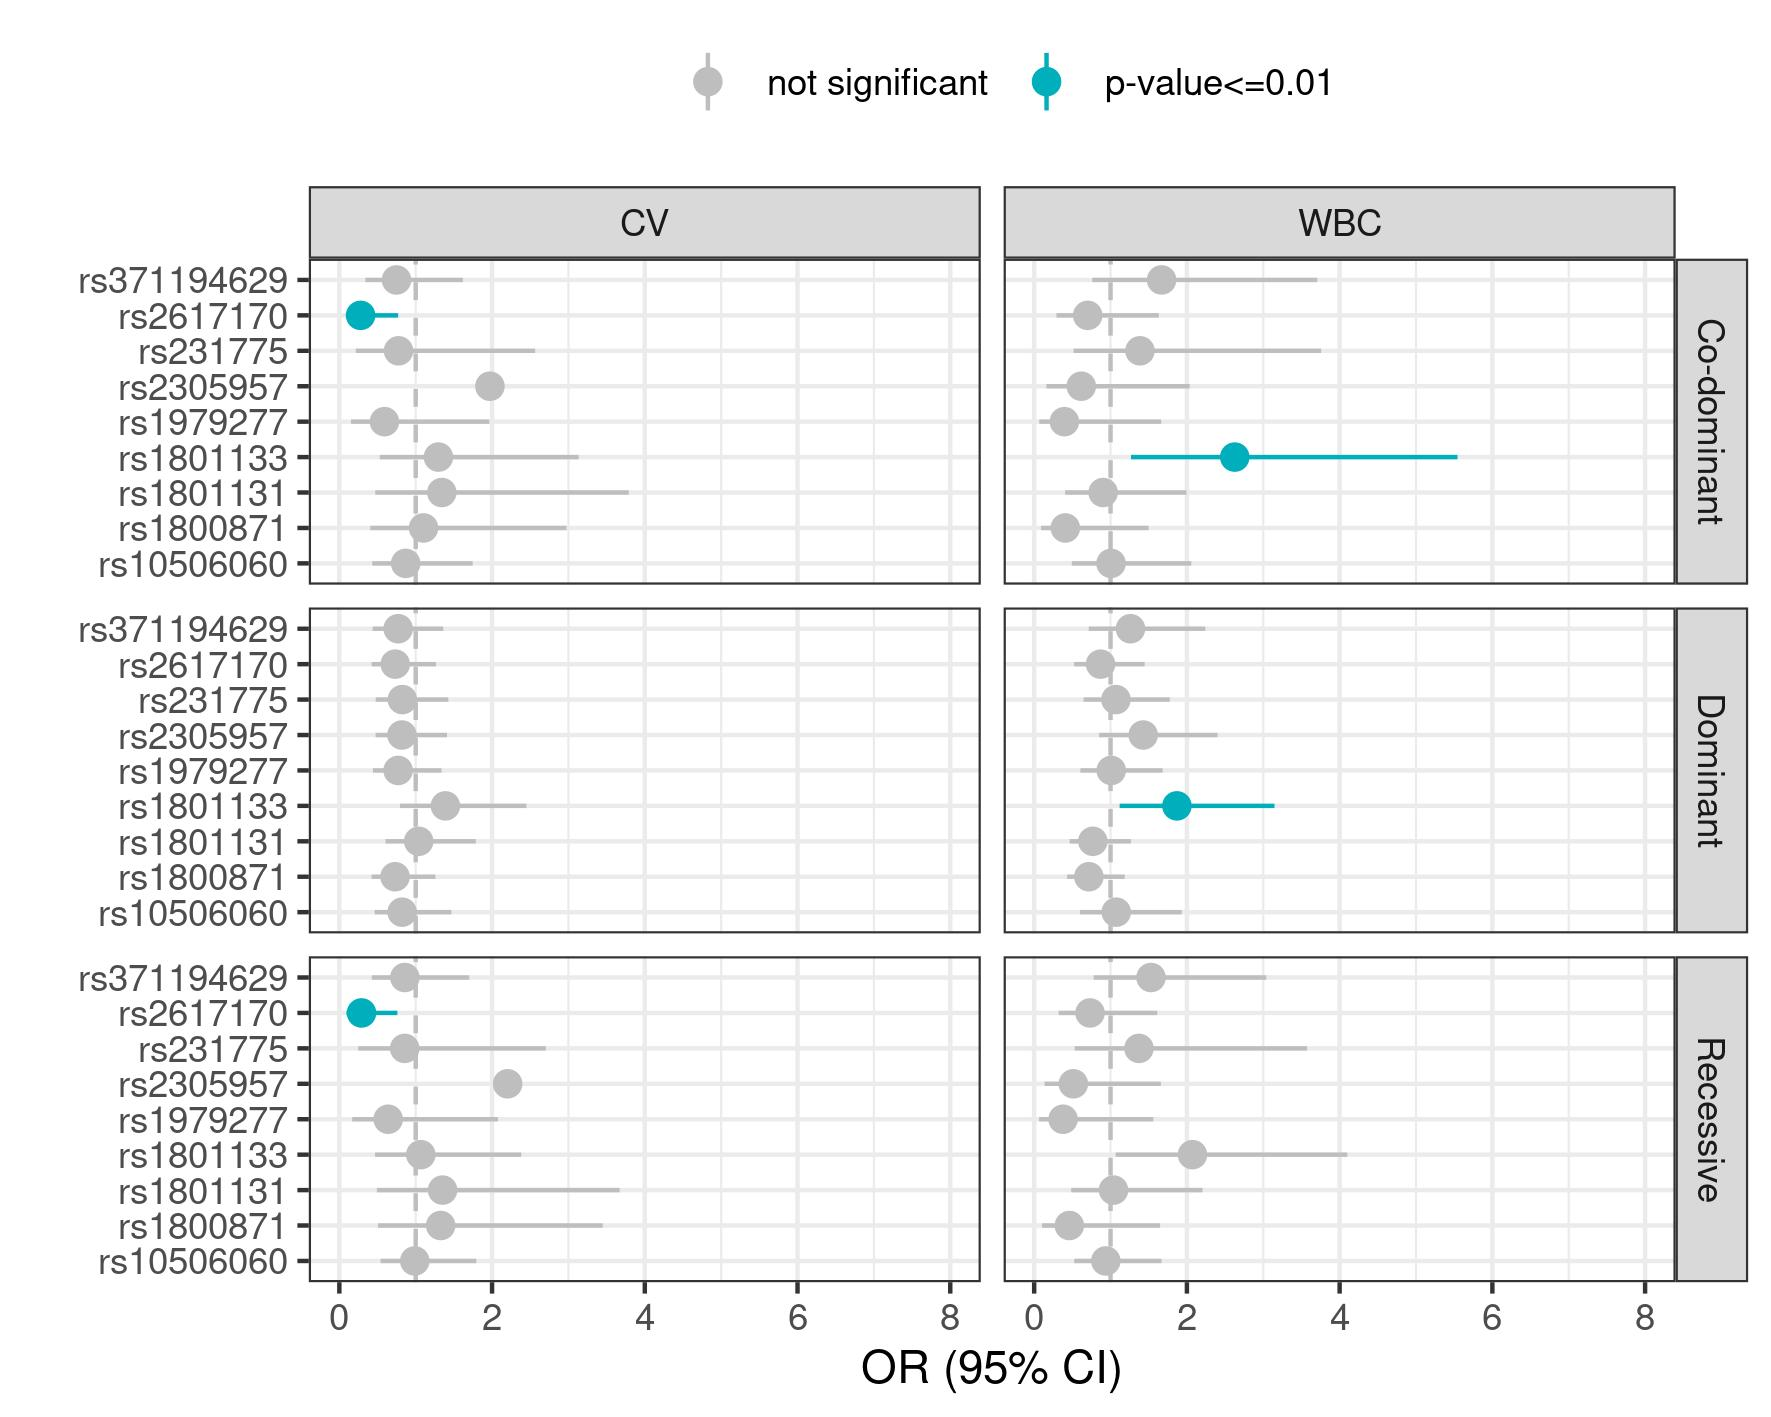
\includegraphics[width=14 cm]{FIGURE/ORgeno.jpg}
    \caption{Genotipic association were explored in three models of disease penetrance: co-dominant, dominant, and recessive both in CV and WBC }
    \label{fig:orgeno}
\end{figure}


\begin{figure}[!ht]
    \centering
    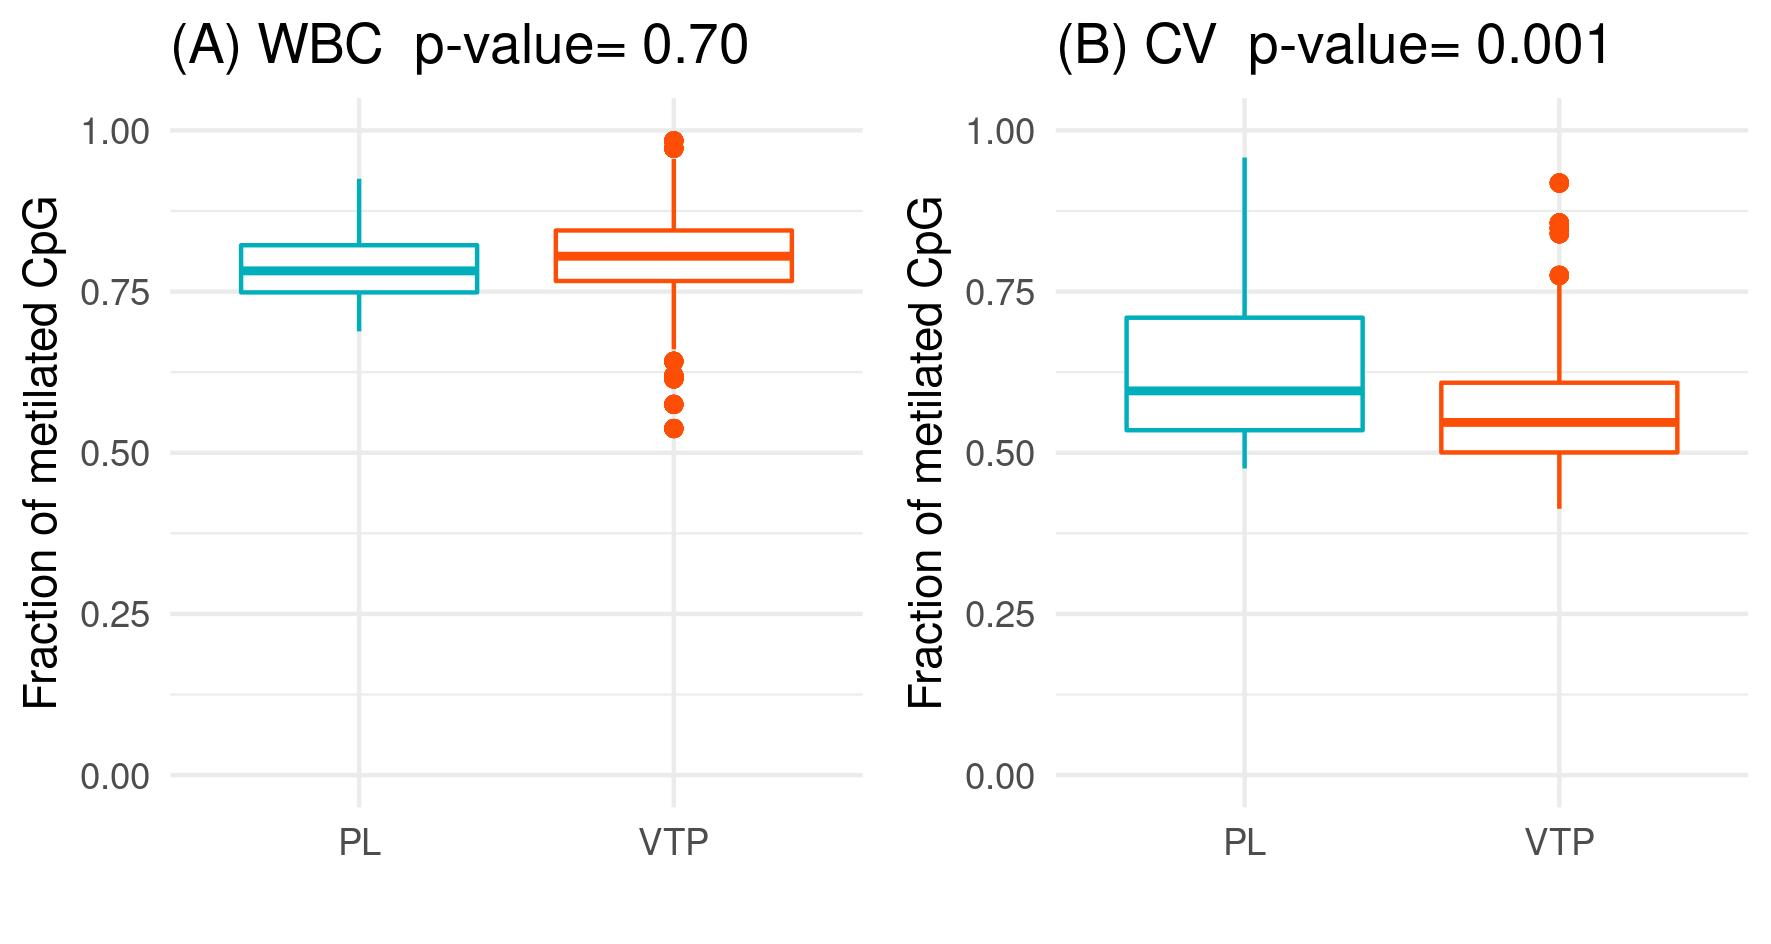
\includegraphics[width=14 cm]{FIGURE/linemet.jpg}
    \caption{Global methylation of LINE-1 in WBC on the left and CV on the right}
    \label{fig:Global methylation}
\end{figure}


\begin{table}[!ht]
\caption{List of genes and variants analyzed in this study}
\centering
 \resizebox{\textwidth}{!}{
\begin{tabular}{ccccccl}
\hline
\textit{\textbf{Gene}} &
  \textit{\textbf{rsID}} &
  \textit{\textbf{Major/minor allele}} &
  \textit{\textbf{\begin{tabular}[c]{@{}c@{}}Chromosome \\ position\end{tabular}}} &
  \multicolumn{1}{c}{\textit{\textbf{Role}}} \\ \hline
MTHFR &
  rs1801133 &
  C/T &
  1:11796321 &
  Metabolism folic acid \cite{liew2015methylenetetrahydrofolate} \\ \hline
MTHFR &
  rs1801131 &
  A/C &
  1:11794419 &
  Metabolism folic acid\cite{kim2006influence} \\ \hline
HLA-G  &
 rs371194629 &
  14bp Del/Ins &
  6:29830804 &
  Immune tolerance in pregnancy \cite{nowak2016possible}\cite{arjmand2016balance}\cite{alassociation} \\ \hline
ANXA5 &
  rs1050606 &
  A/C &
  4:121696891 &
  Ca2+ dependent placenta anticoagulant protein \cite{hayashi2013genotyping} \cite{zhang2017association} \\ \hline
NKG2D &
  rs2617170 &
  A/G &
  12:10408358 &
  Detection and elimination of transformed and infected cells \cite{hizem2014polymorphisms} \\ \hline
IL-10 &
  rs1800871 &
  A/G &
  1:206773289 &
  Cytokines in the cascade of immune signalling \cite{cochery2009interleukin} \cite{qaddourah201410} \\ \hline
CTLA-4 &
  rs231775 &
  A/G &
  2:203867991 &
  Member of immunoglobulin superfamily \cite{misra2016association} \\ \hline
SMTH1 &
  rs1979277 &
  C/T &
  17:18328782 &
  Metabolism folic acid \cite{engel2006polymorphisms} \\ \hline
PLK4 &
  rs2305957 &
  A/G &
  4:127811771 &
  Regulates centriole duplication during cell cycle \cite{zhang2017maternal}\cite{mccoy2015common} \\ \hline
\end{tabular}
}
\label{tab:panelofgenes}
\end{table}



\begin{table}[!ht]
\caption{\textbf{Allelic odds ratios.}Counts of the minor (m) and major (M) alleles are reported. Significant p-values are in \txtbf{bold}.}
\centering 
\resizebox{\textwidth}{!}{%
\begin{tabular}{clllccccl}
\hline
\multicolumn{5}{c}{\textbf{Allele analysis in WBC}} &
  \multicolumn{4}{c}{\textbf{Allele analysis in CV}} \\ \hline
\textit{\textbf{SNP}} &
  \multicolumn{1}{c}{\textit{\textbf{PL}}} &
  \multicolumn{1}{c}{\textit{\textbf{VTP}}} &
  \multicolumn{1}{c}{\textit{\textbf{OR (IC 95\%)}}} &
  \textit{\textbf{p-value}} &
  \textit{\textbf{PL}} &
  \textit{\textbf{VTP}} &
  \textit{\textbf{OR (IC 95\%)}} &
  \multicolumn{1}{c}{\textit{\textbf{p-value}}} \\ \hline
\textit{\textbf{MTHFR rs1801133}} &
   &&& \multicolumn{1}{l}{} & \multicolumn{1}{l}{} & \multicolumn{1}{l}{} &
  \multicolumn{1}{l}{} &\\ \hline
\textit{\textbf{M}} & 138 &207 & & \multicolumn{1}{l}{} &121 &186 & &\\ \hline
\textit{\textbf{m}} &114 & 99 & 1.72(1.22-2.43) & \multicolumn{1}{l}{\textbf{0.0018}} & 81 & 104 & 1.19(0.82-1.73) & \multicolumn{1}{c}{0.33} \\ \hline 
\textit{\textbf{MTHFR rs1801131}} & \multicolumn{1}{c}{} & \multicolumn{1}{c}{} &\multicolumn{1}{c}{} &&\multicolumn{1}{l}{} & \multicolumn{1}{l}{} & \multicolumn{1}{l}{} &\\ \hline
\textit{\textbf{M}} & \multicolumn{1}{c}{173} &\multicolumn{1}{c}{201} & \multicolumn{1}{c}{} & & 138 &205 & & \\ \hline
\textit{\textbf{m}} & \multicolumn{1}{c}{77} & \multicolumn{1}{c}{103} &
\multicolumn{1}{c}{0.86(0.60-1.24)} & 0.44 & 62 & 85 &  1.083(0.73-1.60) &
\multicolumn{1}{c}{0.68} \\ \hline \textit{\textbf{HLA-G 14bp}} & &&&&
 \multicolumn{1}{l}{} & \multicolumn{1}{l}{} & \multicolumn{1}{l}{} &
 \\ \hline \textit{\textbf{M}} & 132 & 161 & &&121 &157 &&
\multicolumn{1}{c}{} \\ \hline \textit{\textbf{m}} & 120 & 137 & 1.068(0.76-1.49) & 0.69 & 81 & 125 & 0.84(0.58-1.21) & \multicolumn{1}{c}{0.35} \\ \hline \textit{\textbf{ANXA5 rs1050606}} & & & && \multicolumn{1}{l}{} &
\multicolumn{1}{l}{} & \multicolumn{1}{l}{} & \\ \hline \textit{\textbf{M}} &
 124 & 148 & & & 107 & 147 & \multicolumn{1}{l}{} & \\ \hline
\textit{\textbf{m}} & 126 & 150 &  1.002(0.71-1.39) & 0.98 & 95 & 143 &
0.91(0.63-1.30) & \multicolumn{1}{c}{0.61} \\ \hline
\textit{\textbf{NKG2D rs2617170}} &&&&& \multicolumn{1}{l}{} & \multicolumn{1}{l}{} & \multicolumn{1}{l}{} & \\ \hline
\textit{\textbf{M}} & 165 & 192 & & & 141 & 174 & \multicolumn{1}{l}{} & \\ \hline \textit{\textbf{m}} & 83 & 112 & 0.86(0.60-1.22) & 0.40 & 61 & 116 & 0.64(0.44-0.95) & \multicolumn{1}{c}{\textbf{0.025}} \\ \hline
\textit{\textbf{IL-10 rs1800871}} &&& && \multicolumn{1}{l}{} & \multicolumn{1}{l}{} &  \multicolumn{1}{l}{} & \\ \hline
\textit{\textbf{M}} & 191 & 210 & & & 143 & 194 & & \\ \hline
\textit{\textbf{m}} & 59 & 88 & 0.73(0.50-1.081) & 0.11 & 57 & 88 & 0.87(0.59-1.30) & \multicolumn{1}{c}{0.52} \\ \hline
\textit{\textbf{CTLA-4 rs231775}} & & & & \multicolumn{1}{l}{} & \multicolumn{1}{l}{} & \multicolumn{1}{l}{} & \multicolumn{1}{l}{} & \\ \hline
\textit{\textbf{M}} & 167 & 211 & & & 139 & 192 & \multicolumn{1}{l}{} &\\ \hline \textit{\textbf{m}} & 81 & 93 & 1.10(0.76-1.57) & 0.60 & 61 & 96 & 0.87(0.60-1.40) & \multicolumn{1}{c}{0.50} \\ \hline \textit{\textbf{SMTH1 rs1979277}} & & & & & & & \multicolumn{1}{l}{} & \\ \hline
\textit{\textbf{M}} & 194 & 223 & & & 155 & 211 & & \\ \hline \textit{\textbf{m}} & 56 & 71 & 0.90(0.60-1.35) & 0.63 & 43 & 75 & 0.78(0.50-1.19) & \multicolumn{1}{c}{0.25} \\ \hline \textit{\textbf{PLK4 rs2305957}} & & & & & & & \multicolumn{1}{l}{} & \\ \hline
\textit{\textbf{M}} & 187 & 226 & & & 153 & 217 & & \\ \hline
\textit{\textbf{m}} & 61 & 64 & 1.15(0.77-1.71) & 0.48 & 47 & 73 & \multicolumn{1}{l}{0.91(0.44-0.95)} & \multicolumn{1}{c}{0.67} \\ \hline
\end{tabular}%
}
\label{tab:Allele analysis in WBC and CV}
\end{table}


\begin{table}[!ht]
\caption{Global LINE-1 methylation level: Mean and standard deviation (SD) for WBC and CV in PL and VTP.}
\centering
\resizebox{\textwidth}{!}{%
\begin{tabular}{ccccc}
\hline
\textit{\textbf{LINE-1 methylation}} & \multicolumn{2}{c}{\textit{\textbf{T student test in WBC}}} & \multicolumn{2}{c}{\textit{\textbf{Mann-Whitney test in CV}}} \\ \hline
                 & \textbf{Mean SD} & \textbf{p-value} & \textbf{Mean SD} & \textbf{p-value} \\ \hline
\textbf{PL}     & 77\% $\pm$ 0.41\%     &                  & 60\% $\pm$ 1.0\%      &                  \\ \hline
\textbf{VTP}     & 78\% $\pm$  0.62\%    &                  & 55\% $\pm$ 0.83\%      &                  \\ \hline
\textbf{PL-VTP} &                  & \textit{p= 0.70} &                  & \textit{\textbf{p=0.0010}} \\ \hline
\end{tabular}%
}
\label{tab:methylation level}
\end{table}



\begin{table}[!ht]
\caption{Evaluation of LINE-1 methylation in subsets based on the clinical data.}
\centering
\resizebox{\textwidth}{!}{%
\begin{tabular}{ccccccc}
\hline
\textit{\textbf{\begin{tabular}[c]{@{}c@{}} LINE-1 \\ methylation\end{tabular}}} &
  \multicolumn{3}{c}{\textit{\textbf{Analysis level of methylation in WBC}}} &
  \multicolumn{3}{c}{\textit{\textbf{Analysis level of methylation in CV}}} \\ \hline
\textit{\textbf{}} &
  \textit{\textbf{Mean $\pm$ SD}} &
  \textit{\textbf{Mean $\pm$ SD}} &
  \textit{\textbf{p-value}} &
  \textit{\textbf{Mean $\pm$ SD}} &
  \textit{\textbf{Mean $\pm$ SD}} &
  \textit{\textbf{p-value}} \\ \hline
\textit{\textbf{Mother's age 35 years}} &
  \textit{\textbf{\textgreater{}=35}} &
  \textit{\textbf{\textless{}35}} &
  \textit{} &
  \textbf{\textgreater{}=35} &
  \textbf{\textless{}35} &
  \textit{} \\ \hline
PL                        & 77 \% \pm  0.40\%       & 78\% \pm 0.40\%     & \textit{p= 0.46} & 61\%  \pm 0.94\%      & 60\%   \pm  1.05\%     & \textit{p=0.53} \\ \hline
VTP                       & 76\%  \pm 0.53 \%          & 78\%   \pm  0.64 \%         & \textit{p=0.20} & 54\% \pm  0.78 \%      & 55\%  \pm  0.86 \%      & \textit{p=0.87} \\ \hline
\textit{\textbf{Mother's BMI}} &
  \textit{\textbf{Normal weight}} &
  \textit{\textbf{Overweight}} &
  \textit{\textbf{}} &
  \textit{\textbf{Normal weight}} &
  \textit{\textbf{Overweight}} &
  \textit{\textbf{}} \\ \hline
PL                        & 78\% \pm 0.37\%  & 76\% \pm 0.48\%           & \textit{p=0.080} & 59\% \pm 1.0 \%        & 62\% \pm   1.0 \%      & \textit{p=0.40} \\ \hline
VTP                       & 78\% \pm  0.54 \%       & 76\%  \pm 0.70 \%       & \textit{p=0.20} & 54\% \pm 0.78 \%         & 55\% \pm   0.76 \%       & \textit{p=0.51} \\ \hline
\textit{\textbf{Smoking exposure}} &
  \textit{\textbf{"Yes"}} &
  \textit{\textbf{"No"}} &
  \textit{\textbf{}} &
  \textit{\textbf{"Yes"}} &
  \textit{\textbf{"No"}} &
   \\ \hline
PL                        & 78\%\pm 0.38 \%     & 77\%\pm 0.39\%    & \textit{p=0.70} & 61\% \pm  1.0\%          & 59\% \pm   0.95\%        & \textit{p=0.59} \\ \hline
VTP                       & 79\% \pm  0.46\%       & 75 \% \pm 0.69\%       & \textit{{p=0.060}} & 54\% \pm    0.89\%       & 54\%  \pm    0.71\%     & \textit{p=0.79} \\ \hline
\textit{\textbf{Embryo's age}} &
  \textit{\textbf{\textgreater{}70}} &
  \textit{\textbf{\textless{}=70}} &
  \textit{\textbf{}} &
  \textit{\textbf{\textgreater{}70}} &
  \textit{\textbf{\textless{}=70}} &
   \\ \hline
PL                        & 78\%  \pm 0.42\%        & 77\% \pm 0.41\%         & \textit{p=0.36} & 58\% \pm  0.9\%        & 62\% \pm 1.0\%         & \textit{p=0.06} \\ \hline
VTP                       & 79\% \pm 0.5\%         & 76\% \pm  0.6\%         & \textit{p= 0.06} & 53\% \pm  0.9\%        & 56\% \pm  0.8\%         & \textit{p=0.10} \\ \hline
\textit{\textbf{Folic acid}} &
  \textit{\textbf{"Yes"}} &
  \textit{\textbf{"No"}} &
  \textit{} &
  \textbf{"Yes"} &
  \textbf{"No"} &
  \textit{} \\ \hline
PL                        & 77\% \pm 0.45\%         & 77\% \pm 0.38 \%          & \textit{p= 0.97} &    57\% \pm 0.81\%     &   62\% \pm 1.0\%       & \textit{\textbf{p= 0.030}} \\ \hline
VTP                       & NA           & NA           & \textit{NA} &  NA         & 78\% \pm 0.56 \%         & \textit{NA} \\ \hline
\textit{\textbf{Embryo's sex}} &
  \textit{\textbf{"Female"}} &
  \textit{\textbf{"Male"}} &
  \textit{\textbf{}} &
  \textit{\textbf{"Female"}} &
  \textit{\textbf{"Male"}} &
  \textit{} \\ \hline
PL                        & 78\% \pm 0.41 \%         & 77\%\pm 0.45 \%          & \textit{p=0.76} & 61\%   \pm  1.0\%     & 60\% \pm 0.80\%         & \textit{p=0.86} \\ \hline
VTP                       & 78\% \pm 0.54\%
& 77 \% \pm 0.67 \%        & \textit{p=0.40} & 56\%  \pm 1.0 \%      & 54\% \pm   0.68 \%       & \textit{p=0.67} \\ \hline
\end{tabular}}
\label{tab:LINE-1 methylation on clinical data}
\end{table}



\nolinenumbers

% Either type in your references using
% \begin{thebibliography}{}
% \bibitem{}
% Text
% \end{thebibliography}
%
% or
%
% Compile your BiBTeX database using our plos2015.bst
% style file and paste the contents of your .bbl file
% here. See http://journals.plos.org/plosone/s/latex for 
% step-by-step instructions.
% 

\bibliography{references} 

%\begin{\bibliography{}{10}

%\bibitem{bib1}
%Conant GC, Wolfe KH.
%\newblock {{T}urning a hobby into a job: how duplicated genes find new
%  functions}.
%\newblock Nat Rev Genet. 2008 Dec;9(12):938--950.

%\bibitem{bib2}
%Ohno S.
%\newblock Evolution by gene duplication.
%\newblock London: George Alien \& Unwin Ltd. Berlin, Heidelberg and New York:
%  Springer-Verlag.; 1970.

%\bibitem{bib3}
%Magwire MM, Bayer F, Webster CL, Cao C, Jiggins FM.
%\newblock {{S}uccessive increases in the resistance of {D}rosophila to viral
%  infection through a transposon insertion followed by a {D}uplication}.
%\newblock PLoS Genet. 2011 Oct;7(10):e1002337.

%\end{thebibliography}

\newpage
\beginsupplement
%%%%%%%%%%%%%%%%%%%%%%%%%
\section*{Supporting information}
\begin{table}[!ht]
\caption{\textbf{Hardy-Weinberg equilibrium test results.} M = major allele, m= minor allele.}
\centering
\resizebox{\textwidth}{!}{%
\begin{tabular}{ccccccccclccccccccc}
\hline
\textit{\textbf{}} &
  \multicolumn{4}{c}{\textit{\textbf{PL WBC}}} &
  \multicolumn{4}{c}{\textit{\textbf{VTP WBC}}} &
  \multicolumn{1}{c}{\textit{\textbf{WBC}}} &
  \multicolumn{4}{c}{\textit{\textbf{PL CV}}} &
  \multicolumn{4}{c}{\textit{\textbf{VTP CV}}} &
  \textit{\textbf{CV}} \\ \hline
\textit{\textbf{SNP}} &
  \textit{\textbf{\begin{tabular}[c]{@{}c@{}}MM\\ (n)\end{tabular}}} &
  \textit{\textbf{\begin{tabular}[c]{@{}c@{}}Mm\\  (n)\end{tabular}}} &
  \textit{\textbf{\begin{tabular}[c]{@{}c@{}}mm\\  (n)\end{tabular}}} &
  \textit{\textbf{\begin{tabular}[c]{@{}c@{}}HWE\\  p-value\end{tabular}}} &
   \textit{\textbf{\begin{tabular}[c]{@{}c@{}}MM\\ (n)\end{tabular}}} &
  \textit{\textbf{\begin{tabular}[c]{@{}c@{}}Mm\\  (n)\end{tabular}}} &
  \textit{\textbf{\begin{tabular}[c]{@{}c@{}}mm\\  (n)\end{tabular}}} &
  \textit{\textbf{\begin{tabular}[c]{@{}c@{}}HWE\\  p-value\end{tabular}}} &
  \multicolumn{1}{c}{\textit{\textbf{\begin{tabular}[c]{@{}c@{}}Total \\ HWE\end{tabular}}}} &
 \textit{\textbf{\begin{tabular}[c]{@{}c@{}}MM\\ (n)\end{tabular}}} &
  \textit{\textbf{\begin{tabular}[c]{@{}c@{}}Mm\\  (n)\end{tabular}}} &
  \textit{\textbf{\begin{tabular}[c]{@{}c@{}}mm\\  (n)\end{tabular}}} &
  \textit{\textbf{\begin{tabular}[c]{@{}c@{}}HWE\\ p-value\end{tabular}}} &
  \textit{\textbf{\begin{tabular}[c]{@{}c@{}}MM\\ (n)\end{tabular}}} &
  \textit{\textbf{\begin{tabular}[c]{@{}c@{}}Mm\\  (n)\end{tabular}}} &
  \textit{\textbf{\begin{tabular}[c]{@{}c@{}}mm\\  (n)\end{tabular}}} &
  \textit{\textbf{\begin{tabular}[c]{@{}c@{}}HWE\\  p-value\end{tabular}}} &
  \textit{\textbf{\begin{tabular}[c]{@{}c@{}}Total\\ HWE\end{tabular}}} \\ \hline
\textit{\textbf{MTHFR rs1801133}} &
  42 &
  54 &
  30 &
  \textit{p= 0.16} &
  74 &
  59 &
  20 &
  \textit{p=0.18} &
  \textit{p=0.05} &
  34 &
  53 &
  14 &
  \textit{p=0.43} &
  60 &
  66 &
  19 &
  \textit{p=0.96} &
  \textit{p=0.70} \\ \hline
\textit{\textbf{MTHFR rs1801131}} &
  65 &
  43 &
  17 &
  \textit{p=0.050} &
  69 &
  63 &
  20 &
  \textit{p=0.43} &
  \textit{p=0.05} &
  48 &
  42 &
  10 &
  \textit{p=0.95} &
  71 &
  63 &
  11 &
  \textit{p=0.66} &
  \textit{p=0.83} \\ \hline
\textit{\textbf{HLA-G 14 bp}} &
  33 &
  66 &
  27 &
  \textit{p=0.66} &
  43 &
  75 &
  31 &
  \textit{p=0.95} &
  \textit{p=0.68} &
  39 &
  43 &
  19 &
  \textit{p=0.32} &
  46 &
  65 &
  30 &
  \textit{p=0.51} &
  \textit{p=0.20} \\ \hline
\textit{\textbf{ANXA5 rs1050606}} &
  31 &
  62 &
  32 &
  \textit{p=0.94} &
  39 &
  70 &
  40 &
  \textit{p=0.53} &
  \textit{p=0.60} &
  35 &
  37 &
  29 &
  \textit{p=0.012} &
  44 &
  59 &
  42 &
  \textit{p=0.034} &
  \textit{p=0.050} \\ \hline
\textit{\textbf{NKG2D rs2617170}} &
  54 &
  57 &
  13 &
  \textit{p=0.83} &
  61 &
  70 &
  21 &
  \textit{p=0.96} &
  \textit{p=0.97} &
  46 &
  49 &
  6 &
  \textit{p=0.18} &
  55 &
  64 &
  26 &
  \textit{p=0.40} &
  \textit{p=0.94} \\ \hline
\textit{\textbf{IL-10 rs1800871}} &
  70 &
  51 &
  4 &
  \textit{p=0.20} &
  71 &
  68 &
  10 &
  \textit{p=0.30} &
  \textit{p=0.10} &
  54 &
  35 &
  11 &
  \textit{p=0.22} &
  65 &
  64 &
  12 &
  \textit{p=0.59} &
  \multicolumn{1}{l}{\textit{p=0.80}} \\ \hline
\textit{\textbf{CTLA-4 rs231775}} &
  55 &
  57 &
  12 &
  \textit{p=0.72} &
  70 &
  71 &
  11 &
  \textit{p=0.27} &
  \textit{p=0.26} &
  45 &
  49 &
  6 &
  \textit{p=0.16} &
  58 &
  76 &
  10 &
  \textit{p=0.040} &
  \multicolumn{1}{l}{\textit{p=0.10}} \\ \hline
\textit{\textbf{SMTH1 rs1979277}} &
  72 &
  50 &
  3 &
  \textit{p=0.14} &
  85 &
  53 &
  9 &
  \textit{p=0.95} &
  \textit{p=0.41} &
  61 &
  33 &
  5 &
  \textit{p=0.93} &
  79 &
  53 &
  11 &
  \textit{p=0.73} &
  \multicolumn{1}{l}{p=0.67} \\ \hline
\textit{\textbf{PLK4 rs2305957}} &
  68 &
  51 &
  5 &
  \textit{p=0.30} &
  92 &
  42 &
  11 &
  \textit{p=0.010} &
  \textit{p=0.71} &
  56 &
  41 &
  3 &
  \textit{p=0.23} &
  74 &
  69 &
  2 &
  \textit{p=0.030} &
  \multicolumn{1}{l}{p=0.055} \\ \hline
\end{tabular}%
}
\label{tab:HWE in WBC and CV}
\end{table}

\begin{table}[!ht]
\caption{\textbf{Genotypic odds ratio}, confidence intervals, and p-values under co-dominant, dominant, and recessive models of disease penetrance. m=minor allele, M=major allele. Significant associations are in \textbf{bold}.} 
    \centering
    \begin{tabular}{llllllll}
\hline
\multicolumn{1}{c}{\textit{\textbf{Model}}} &
  \multicolumn{1}{c}{\textit{\textbf{Sample}}} &
  \textit{\textbf{Gene}} &
  \textit{\textbf{SNP}} &
  \textit{\textbf{OR}} &
  \textit{\textbf{lowCI}} &
  \textit{\textbf{highCI}} &
  \textit{\textbf{pval}} \\ \hline\multicolumn{1}{c}{\multirow{9}{*}{\textit{Dominant}}} &
  \multicolumn{1}{c}{\multirow{9}{*}{WBC}} & \textbf{MTHFR} &
  \textbf{rs1801133} &
  \textbf{1.87} &
  \textbf{1.12} &
  \textbf{3.15} &
  \textbf{0.01451} \\ \cline{3-8} 
\multicolumn{1}{c}{} & \multicolumn{1}{c}{} & MTHFR          & rs1801131          & 0.77          & 0.46          & 1.27          & 0.27997          \\ \cline{3-8} 
\multicolumn{1}{c}{} & \multicolumn{1}{c}{} & HLAG           & rs371194629        & 1.26          & 0.71          & 2.24          & 0.41702          \\ \cline{3-8} 
\multicolumn{1}{c}{} & \multicolumn{1}{c}{} & ANXA5          & rs10506060         & 1.07          & 0.60          & 1.93          & 0.88952          \\ \cline{3-8} 
\multicolumn{1}{c}{} & \multicolumn{1}{c}{} & NKG2D          & rs2617170          & 0.87          & 0.52          & 1.45          & 0.62385          \\ \cline{3-8} 
\multicolumn{1}{c}{} & \multicolumn{1}{c}{} & IL-10          & rs1800871          & 0.72          & 0.43          & 1.19          & 0.18321          \\ \cline{3-8} 
\multicolumn{1}{c}{} & \multicolumn{1}{c}{} & CTLA-4         & rs231775           & 1.07          & 0.65          & 1.77          & 0.80865          \\ \cline{3-8} 
\multicolumn{1}{c}{} & \multicolumn{1}{c}{} & SMTH1          & rs1979277          & 1.01          & 0.60          & 1.68          & 1.00000          \\ \cline{3-8} 
\multicolumn{1}{c}{} & \multicolumn{1}{c}{} & PLK4           & rs2305957          & 1.43          & 0.85          & 2.40          & 0.17123          \\ \hline
\multirow{9}{*}{}    & \multirow{9}{*}{CV}  & MTHFR          & rs1801133          & 1.39          & 0.79          & 2.45          & 0.23282          \\ \cline{3-8} 
 &                      & MTHFR          & rs1801131          & 1.04          & 0.60  & 1.79          & 0.89722          \\ \cline{3-8} 
 &                      & HLAG           & rs371194629        & 0.77          & 0.44  & 1.36          & 0.34296          \\ \cline{3-8} 
&                      & ANXA5          & rs10506060         & 0.82          & 0.46   & 1.47          & 0.49062          \\ \cline{3-8} 
 &                      & NKG2D          & rs2617170          & 0.73          & 0.42  & 1.27          & 0.23913          \\ \cline{3-8} 
 &                      & IL-10          & rs1800871          & 0.73          & 0.42  & 1.26          & 0.24152          \\ \cline{3-8} 
 &                      & CTLA-4         & rs231775           & 0.82          & 0.48  & 1.43          & 0.51066          \\ \cline{3-8} 
 &                      & SMTH1          & rs1979277          & 0.77          & 0.44  & 1.34          & 0.35546          \\ \cline{3-8} 
 &   & PLK4           & rs2305957          & 0.82          & 0.47          & 1.41     & 0.51511          \\ \hline
 \multirow{9}{*}{\textit{Recessive}} &
  \multirow{9}{*}{WBC} &
  \textbf{MTHFR} &
  \textbf{rs1801133} &
  \textbf{2.07} &
  \textbf{1.07} &
  \textbf{4.10} &
  \textbf{0.02749} \\ \cline{3-8} 
 &   & MTHFR          & rs1801131          & 1.04          & 0.48          & 2.20    & 1.00000          \\ \cline{3-8} 
  &                      & HLAG           & rs371194629        & 1.53          & 0.78  & 3.04          & 0.20336 \\ \cline{3-8}  &   & ANXA5          & rs10506060         & 0.94          & 0.53          & 1.67 & 0.89061          \\ \cline{3-8} 
 &                      & NKG2D          & rs2617170          & 0.73          & 0.32 & 1.61          & 0.46387          \\ \cline{3-8} 
&   & IL-10          & rs1800871          & 0.46          & 0.10          & 1.65          & 0.27160          \\ \cline{3-8} 
 &                      & CTLA-4         & rs231775           & 1.37          & 0.53  & 3.57          & 0.51560          \\ \cline{3-8} 
 &   & SMTH1          & rs1979277          & 0.38          & 0.06          & 1.56     & 0.15302          \\ \cline{3-8} 
 &                      & PLK4           & rs2305957          & 0.51          & 0.14  & 1.66          & 0.30239          \\ \hline
\multirow{9}{*}{}  & \multirow{9}{*}{CV}  & MTHFR          & rs1801133          & 1.07          & 0.47          & 2.38          & 0.85192          \\ \cline{3-8} 
&                      & MTHFR          & rs1801131          & 1.35          & 0.49   & 3.67          & 0.64324          \\ \cline{3-8} 
 & & HLAG           & rs371194629        & 0.86          & 0.42          & 1.70       & 0.74600          \\ \cline{3-8} 
 &   & ANXA5          & rs10506060         & 0.99          & 0.54          & 1.79    & 1.00000          \\ \cline{3-8} 
 &  & \textbf{NKG2D} & \textbf{rs2617170} & \textbf{0.29} & \textbf{0.09} & \textbf{0.76} & \textbf{0.00652} \\ \cline{3-8} 
 &   & IL-10          & rs1800871          & 1.33          & 0.51          & 3.45     & 0.51477          \\ \cline{3-8} 
 &  & CTLA-4         & rs231775           & 0.86          & 0.25          & 2.70      & 1.00000   \\ \cline{3-8} 
&  & SMTH1  & rs1979277   & 0.64  & 0.17   & 2.08 & 0.59999          \\ \cline{3-8} 
 &   & PLK4           & rs2305957          & 2.20          & 0.25          & 26.85    & 0.40087  \\ \hline
 \multirow{9}{*}{\textit{Co-dominant}} &
  \multirow{9}{*}{WBC} &
  \textbf{MTHFR} &
  \textbf{rs1801133} &
  \textbf{2.63} &
  \textbf{1.27} &
  \textbf{5.54} &
  \textbf{0.00616} \\ \cline{3-8} 
&  & MTHFR          & rs1801131          & 0.90   & 0.41          & 1.99          & 0.85347          \\ \cline{3-8} 
 &   & HLAG           & rs371194629        & 1.67          & 0.76          & 3.71    & 0.19793          \\ \cline{3-8} 
&   & ANXA5          & rs10506060         & 1.01          & 0.49          & 2.06          & 1.00000  \\ \cline{3-8} 
&   & NKG2D   & rs2617170          & 0.70          & 0.29          & 1.63       & 0.43476    \\ \cline{3-8} 
&  & IL-10          & rs1800871          & 0.41   & 0.09          & 1.50          & 0.16584   \\ \cline{3-8} 
&  & CTLA-4  & rs231775 & 1.39          & 0.52  & 3.76  & 0.50128     \\ \cline{3-8} 
&   & SMTH1  & rs1979277          & 0.40    & 0.07          & 1.66          & 0.23027  \\ \cline{3-8} 
&   & PLK4   & rs2305957     & 0.62          & 0.16  & 2.04     & 0.43669          \\ \hline
\multirow{9}{*}{} & \multirow{9}{*}{CV}  & MTHFR & rs1801133  & 1.30 & 0.53   & 3.13  & 0.53794          \\ \cline{3-8} 
 &   & MTHFR  & rs1801131  & 1.34          & 0.47   & 3.79  & 0.63244          \\ \cline{3-8} 
&  & HLAG  & rs371194629 & 0.75  & 0.34    & 1.62  & 0.47195  \\ \cline{3-8} 
  &  & ANXA5 & rs10506060         & 0.87   & 0.43 & 1.75          & 0.74166 \\ \cline{3-8} 
&  & \textbf{NKG2D} & \textbf{rs2617170} & \textbf{0.28} & \textbf{0.09} & \textbf{0.77} & \textbf{0.00705} \\ \cline{3-8} 
 &  & IL-10          & rs1800871          & 1.10  & 0.41          & 2.97          & 1.00000     \\ \cline{3-8} 
 &   & CTLA-4         & rs231775           & 0.77          & 0.21          & 2.56     & 0.78794          \\ \cline{3-8} 
 &  & SMTH1          & rs1979277          & 0.59  & 0.15          & 1.96          & 0.42883 \\ \cline{3-8} 
 &  & PLK4 & rs2305957  & 1.97 & 0.22 & 24.36 & 0.65306          \\ \hline
\end{tabular}
\label{tab:tab:Model genetic analysis in WBC and CV}
\end{table}

\begin{table}[!ht]
\centering
\caption{Genotipic counts at the genomic loci considered. PL=Pregnanacy loss; VTP= voluntary termination of pregnancy; WBC= white blood cells from mothers; CV= chorionic villi from embryos. }
\label{tab:genotipic_count}
\resizebox{\textwidth}{!}{%
\begin{tabular}{lllllllll}
\hline
\textbf{Sample} & \textbf{Gene} & \textbf{SNP} & \textbf{PLmm} & \textbf{VTPmm} & \textbf{PLMm} & \textbf{VTPMm} & \textbf{PLMM} & \textbf{VTPMM} \\ \hline
\multirow{9}{*}{WBC} & MTHFR  & rs1801133   & 30 & 20 & 54 & 59 & 42 & 74 \\ \cline{2-9} 
                     & MTHFR  & rs1801131   & 17 & 20 & 43 & 63 & 65 & 69 \\ \cline{2-9} 
                     & HLAG   & rs371194629 & 27 & 21 & 66 & 75 & 33 & 43 \\ \cline{2-9} 
                     & ANXA5  & rs10506060  & 32 & 40 & 62 & 70 & 31 & 39 \\ \cline{2-9} 
                     & NKG2D  & rs2617170   & 13 & 21 & 57 & 70 & 54 & 61 \\ \cline{2-9} 
                     & IL-10  & rs1800871   & 4  & 10 & 51 & 68 & 70 & 71 \\ \cline{2-9} 
                     & CTLA-4 & rs231775    & 12 & 11 & 57 & 71 & 55 & 70 \\ \cline{2-9} 
                     & SMTH1  & rs1979277   & 3  & 9  & 50 & 53 & 72 & 85 \\ \cline{2-9} 
                     & PLK4   & rs2305957   & 5  & 11 & 51 & 42 & 68 & 92 \\ \hline
\multirow{9}{*}{CV}  & MTHFR  & rs1801133   & 14 & 19 & 53 & 66 & 34 & 60 \\ \cline{2-9} 
                     & MTHFR  & rs1801131   & 10 & 11 & 42 & 63 & 48 & 71 \\ \cline{2-9} 
                     & HLAG   & rs371194629 & 19 & 30 & 43 & 65 & 39 & 46 \\ \cline{2-9} 
                     & ANXA5  & rs10506060  & 29 & 42 & 37 & 59 & 35 & 44 \\ \cline{2-9} 
                     & NKG2D  & rs2617170   & 6  & 26 & 49 & 64 & 46 & 55 \\ \cline{2-9} 
                     & IL-10  & rs1800871   & 11 & 12 & 35 & 64 & 54 & 65 \\ \cline{2-9} 
                     & CTLA-4 & rs231775    & 6  & 10 & 49 & 76 & 45 & 58 \\ \cline{2-9} 
                     & SMTH1  & rs1979277   & 5  & 11 & 33 & 53 & 61 & 79 \\ \cline{2-9} 
                     & PLK4   & rs2305957   & 3  & 2  & 41 & 69 & 56 & 74 \\ \hline
\end{tabular}%
}
\end{table}


%%%%%%%%%%%%%%%%%%%%%%%%%%


\end{document}

